\section{How to deal with and record change requests}
\begin{itemize}
    \item A project manager needs to balance 2 things:
        \begin{enumerate}
            \item The need for change and adaptation to the project needs.
            \item Efficiently manage them in a way that the project is not delayed or affected in terms of cost.
        \end{enumerate}
    
    \item A good PM cannot be stubborn, the PM needs to adapt but the PM also has a buget and needs to keep true to the original estimations.
    \item We have been limiting the potential for change through comprehensive planning. But PM is not perfect, and change needs to be taken into account.
    \item Thus we have special requests called change requests that we can recieve in order to consider a change. A change is being requsted and requests need to be analysed, a change request must contain:
        \begin{itemize}
            \item What are the benefits of the change?
            \item What is needed in order to implement the change?
            \item What is its impact on the project?
        \end{itemize}
    
    \item If the PM thinks the change request makes sense then the proposal will be sent for approval to the project sponsor (since they have provided the resources and therefore determies if th additional needs are worth it). A change request form looks like this:
        \begin{figure}[H]
            \centering
            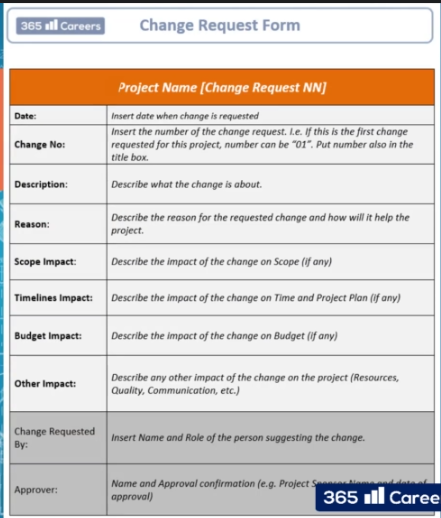
\includegraphics[width=\width\textwidth]{./figs/20221027162453.png}
            %\caption{}
        \end{figure}
    
    \item The PM must then convince the project sponsor that the change will benefit the project. There maybe sometimes where the project sponsor sees no benefit in the additional needs. It is possible that the project can be cancelled if the additional resources are substantial and crucial.
    \item If the change request is approved by the PM and the project sponsor then the PM must check which areas are impacted and how (schedule, budget, scope, resoures, quality, etc.), the changer are of benefit to the project and the sponsor approves the change request.
    \item The PM will be the one to decide if a change that's proposed needs to actually go through this rigorous process.
    \item A team member requesting a couple of days off will not cost additional resouces and will be covered by the buffer.
    \item Remember the scope statement is the best defence against a project not meeting a stakeholder's expectations. If a stakeholder says that the project is not up to his expectations, then the PM can pull out the scope statement and tell the stakeholder that the project was agreed upon by the criteria outlined in the scope statement. If the something crucial is missing then the change request is likely to be initiated, however if the stakholder does not have a point then it will not.
\end{itemize}

\subsection{Planning phase complete recap}
\begin{itemize}
    \item Now you know all of the following components.
        \begin{figure}[H]
            \centering
            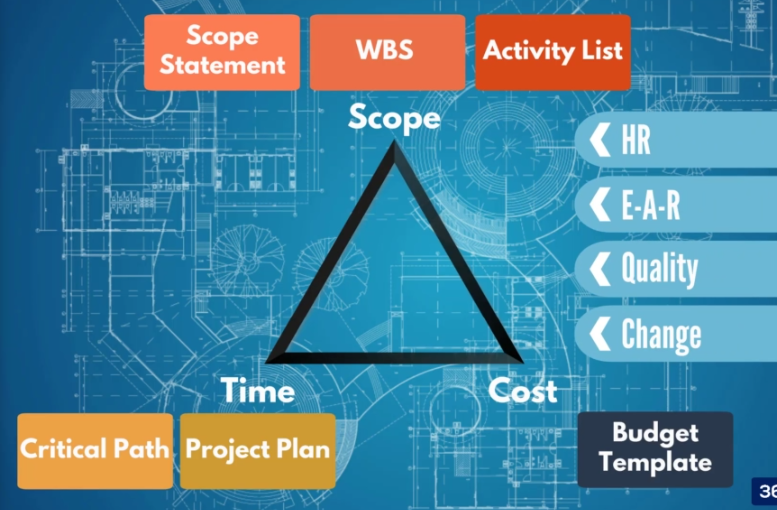
\includegraphics[width=\width\textwidth]{./figs/20221027164646.png}
            %\caption{}
        \end{figure}
    
    \item If a PM wants to complete the project successfully within time and budget then they must put sufficient time, attention, care and effort into the planning. The more things they miss in the planning the higher the chances of changes which will cause delays and harm to the project.
    \item Planning involves many non-straight forward tasks which means the PM must deal with the stakeholders to get the information to build solid assumptions and plans.
    \item Take into account that planning is iterative, new information must be constantly updated. Meaning the PM must go back and update plans.
    \item The PM is responsable for:
        \begin{itemize}
            \item Understand the project.
            \item Identify the important sections.
            \item Investing the appropriate amount of time to plan each section.
            \item Consider all dependencies.
        \end{itemize}
    
    \item They must gather all the data from stakeholders and put it into the scope statement.
    \item Once the PM has identified the expectations for a project, the PM must resolve any discrepancies. 
    \item The PM must finalize and formalise the plan and present it to the project sponsor for approval.
\end{itemize}